% !TEX root = ../main.tex
\chapter{Resultados y Evaluación Logística}
\label{chap:resultados}

Este capítulo presenta el análisis empírico de la ejecución del sistema sobre el dataset \textit{Fresh RetailNet}. Los resultados se organizan en cuatro niveles de evaluación: métricas predictivas, calibración conformal, evaluación económica bajo un \textit{ground truth} común y explicabilidad. El capítulo cierra con una verificación explícita de los KPIs definidos en el Capítulo~\ref{chap:introduccion}.

\textbf{Nota sobre el diseño experimental:} Es fundamental remarcar que la selección del modelo campeón y la evaluación del impacto de la corrección de censura se realizan deliberadamente sobre un \textbf{subset base de 50 series de alta rotación} (las de mayor volumen de ventas histórico). Este subset actúa como un entorno de laboratorio diseñado específicamente para aislar el problema central de esta tesis allí donde tiene mayor impacto económico: los SKUs top ventas, en los que cualquier rotura de stock genera una penalización severa en coste. La posterior validación a escala con 500 series (que introduce la larga cola de productos de menor rotación) se usa únicamente para evaluar la estabilidad estadística de la \textit{Conformal Prediction} (Sección~\ref{sec:resultados_escala}). Evaluar la política de imputación promediando sobre 500 series diluiría el beneficio de la corrección bajo una enorme masa de productos de ventas bajas (donde las roturas apenas suponen pérdidas de 1 o 2 unidades), ocultando el valor logístico del modelo en los productos estratégicos. Los dos protocolos de censura sintética constituyen la excepción a este esquema y operan sobre sus propios subconjuntos, indicados explícitamente en cada caso: 500 series para el error de reconstrucción (Sección~\ref{sec:imputacion_censura_sintetica}) y 30 series para la evaluación de coste justo (Sección~\ref{sec:resultados_gemelo}), al no requerir ninguno de los dos el entrenamiento del modelo de \textit{forecasting}.

\section{Métricas Predictivas y la Trampa del MAE}
\label{sec:resultados_predictivos}

Este bloque evalúa el rendimiento predictivo del sistema y la coherencia de la imputación de demanda censurada a través de tres aproximaciones: una evaluación walk-forward de forecasting, una comparativa downstream de imputadores y una validación directa con censura sintética.

\subsection{Rendimiento Predictivo en el Backtesting Walk-Forward}
\label{sec:predictivo_walkforward}

Esta sección evalúa el rendimiento predictivo puro de los modelos desarrollados. La Tabla~\ref{tab:metrics_predictive} recoge las métricas de error (MAE y RMSE) obtenidas durante el backtesting \textit{walk-forward} con $K=3$ \textit{folds} y un horizonte de $H=7$ días, comparando el rendimiento sobre las ventas observadas frente a la estimación de demanda latente. Las cifras corresponden al panel de \textbf{500 series} (10.500 observaciones de evaluación por combinación modelo-estrategia), el mismo \textit{run} que respalda la calibración conformal a escala de la Sección~\ref{sec:resultados_escala} y los costes simulados que de ella se derivan, de modo que las tres lecturas comparten una única ejecución y son comparables entre sí.

\begin{table}[h]
\centering
\caption{Comparativa de errores predictivos en el backtesting walk-forward ($K=3$ folds, $H=7$ días). Cada estrategia se mide contra su propio target, por lo que los errores no son comparables entre estrategias (véase la discusión en la Sección~\ref{sec:predictivo_walkforward}).}
\label{tab:metrics_predictive}
\begin{tabular}{@{}llcc@{}}
\toprule
Estrategia & Modelo & MAE & RMSE \\
\midrule
Latent Supervised & Seasonal Naïve & 4,47 & 6,05 \\
Latent Supervised & LightGBM & 7,22 & 10,63 \\
Latent Supervised & CatBoost & 7,89 & 10,78 \\
Observed & Seasonal Naïve & 8,73 & 11,82 \\
Observed & CatBoost & 12,91 & 18,28 \\
Observed & LightGBM & 13,71 & 19,76 \\
\bottomrule
\end{tabular}
\end{table}


Al analizar los resultados de la tabla, el fenómeno más llamativo, y pedagógicamente central, es que el modelo heurístico \textit{Seasonal Naïve} obtiene el \textbf{mejor MAE bajo la estrategia de Demanda Latente} (4,47 frente a 5{,}91 de LightGBM y 6{,}91 de CatBoost). Este resultado empírico reproduce y confirma la limitación advertida teóricamente en el Capítulo~\ref{chap:estado_del_arte}: la métrica MAE favorece sistemáticamente a los modelos conservadores que predicen cerca de la mediana histórica, penalizando a los modelos probabilísticos de Machine Learning que estiman los cuantiles extremos (colas de la distribución) necesarios para la optimización logística del modelo \textit{Newsvendor}.

Por otro lado, la corrección de la demanda censurada tiene un efecto consistente y significativo sobre la precisión pura: todos los modelos mejoran sustancialmente su MAE y RMSE cuando se entrenan sobre la estimación de la demanda latente en lugar de las ventas observadas sin procesar. En concreto, CatBoost pasa de un MAE=12{,}26 (Observed) a 6{,}91 (Latent Supervised), lo que supone una drástica reducción del error del 43{,}6\,\%.

No obstante, es fundamental contextualizar este resultado desde una perspectiva metodológica. Desde el punto de vista del negocio y del diseño del sistema, la estimación de la demanda latente (estrategia \textit{Latent Supervised}) constituye el target teóricamente correcto al que debe aspirar el modelo, dado que representa el volumen real de ventas que se habría materializado si no hubiese existido restricción de inventario. En cambio, el target de la estrategia \textit{Observed} está artificialmente sesgado a la baja por los periodos de rotura. Sin embargo, para la evaluación estadística de los errores (MAE y RMSE) en esta tabla, cada modelo se mide contra su propio target de entrenamiento (las ventas observadas para la estrategia \textit{Observed}, y la señal imputada y suavizada para \textit{Latent Supervised}). Esto impide realizar una comparación directa de errores predictivos (un problema de comparar ``peras con manzanas''), dado que predecir una señal reconstruida y suavizada es matemáticamente más sencillo que predecir las ventas reales directas con caídas bruscas a cero. Por tanto, la Tabla~\ref{tab:metrics_predictive} demuestra la coherencia interna de los modelos entrenados con datos corregidos, pero la validez externa del método y su capacidad de reconstrucción de la señal real se demuestran de forma rigurosa mediante la censura sintética y la optimización de costes en las secciones siguientes (Secciones~\ref{sec:resultados_imputacion} y~\ref{sec:resultados_gemelo}).



\subsection{Las Tres Estrategias de Imputación y sus Dos Rutas de Evaluación}
\label{sec:resultados_imputacion}

El módulo \texttt{LatentDemandImputer} implementa tres estrategias de imputación alternativas (véase Sección~\ref{sec:demanda_censurada}): un escalado proporcional fijo (\textit{Clipped Scaling}, $\gamma = 1{,}2$), la media histórica local de la serie y una estimación supervisada con LightGBM condicionada a las covariables del día. Elegir entre ellas exige decidir \emph{contra qué} se las mide, y este trabajo las evalúa por dos rutas metodológicamente independientes:

\begin{itemize}
    \item \textbf{Fidelidad de reconstrucción} (directa): cuánto se acerca la señal imputada a la demanda real, medida sobre días limpios censurados artificialmente, donde esa demanda sí se conoce. Es la Sección~\ref{sec:imputacion_censura_sintetica}.
    \item \textbf{Utilidad económica} (\textit{downstream}): cuánto coste de inventario induce cada señal cuando alimenta la política de pedido, con todas las estrategias puntuadas contra una misma demanda real. Es la evaluación de coste justo de la Sección~\ref{sec:resultados_gemelo}.
\end{itemize}

Ambas rutas convergen en la estrategia Supervisada, y el interés está en que \emph{no} coinciden en el orden de las dos heurísticas: la discusión de esa discrepancia se aborda en la Sección~\ref{sec:resultados_gemelo}, donde se dispone de las dos tablas para contrastarlas.

Una tercera ruta, la de comparar las estrategias por el Winkler Score del modelo de \textit{forecasting} entrenado sobre cada señal, se exploró en una iteración anterior del sistema, pero no se reporta aquí: el punto de entrada actual \texttt{run\_imputation\_comparison()} es deliberadamente previo al modelado (no entrena modelos ni ejecuta \textit{folds}), de modo que esas cifras no son reproducibles con el código de esta versión y no superan la regla de trazabilidad que se aplica al resto del capítulo (todo número citado debe nombrar el \textit{run} y el \textit{commit} que lo produjo). Se omite antes que reportar una cifra que no puede auditarse hasta su artefacto.

Sí conviene anticipar el mecanismo que distingue a las tres, porque explica los resultados de ambas rutas. El \textit{Clipped Scaling} escala uniformemente un 20\% la demanda observada, de modo que introduce ruido en días con stockouts cortos (1--2 horas), donde la corrección necesaria es mínima, y se queda muy corto en las roturas severas; de ahí su sesgo estructural negativo. La media histórica local ignora igualmente la severidad, pero en el sentido contrario: imputa el nivel medio de la serie con independencia de si la rotura duró una hora o doce. La estrategia Supervisada evita ambos problemas al estimar la corrección de forma condicional a las covariables del día (ratio de stockout, media histórica de la serie, calendario y variables meteorológicas), lo que le permite hacer una imputación proporcionada a la severidad real de cada rotura de stock.

\subsection{Evaluación Directa mediante Censura Sintética}
\label{sec:imputacion_censura_sintetica}

La ruta económica de la sección anterior es una evaluación \textit{indirecta}: mide la calidad de cada estrategia a través de las decisiones que induce. Medir directamente el error de reconstrucción tropieza con una limitación conceptual de fondo: la demanda latente en un día con rotura real es un \textbf{contrafactual no observable}, ya que nunca se conoce cuánto se habría vendido con disponibilidad plena, por lo que sobre esos días no existe verdad-terreno alguna contra la que comparar.

Para sortear esta imposibilidad se diseña un protocolo de \textbf{censura sintética} sobre los días limpios, donde la demanda real sí es conocida. El procedimiento es: (i) se reserva un subconjunto aleatorio del 30\% de los días sin rotura (\texttt{stockout\_hours}~$=0$); (ii) a cada día reservado se le asigna un ratio de rotura muestreado de la \textbf{distribución empírica de los stockouts reales} del panel, y se reduce su venta de forma proporcional ($\text{venta}_{\text{censurada}} = \text{demanda}_{\text{real}}\cdot(1-r)$), simulando así una rotura realista; (iii) cada estrategia reconstruye esos días censurados artificialmente; y (iv) se compara la estimación contra la demanda real conocida. La Tabla~\ref{tab:imputation_reconstruction} recoge el error de reconstrucción sobre $n=5\,009$ días censurados sintéticamente en el panel de 500 series.

\begin{table}[h]
\centering
\caption{Error directo de reconstrucción por censura sintética sobre días limpios ($n=5\,009$, panel de 500 series). MAE/RMSE menores y sesgo próximo a cero indican mejor reconstrucción.}
\label{tab:imputation_reconstruction}
\begin{tabular}{lrrrr}
\toprule
\textbf{Estrategia} & \textbf{MAE} & \textbf{RMSE} & \textbf{Sesgo} & \textbf{MAPE} \\
\midrule
\textbf{Supervisada (LightGBM)} & \textbf{1{,}11} & \textbf{1{,}55} & \textbf{$+$0{,}03} & \textbf{16{,}5\%} \\
Media Histórica Local & 1{,}62 & 2{,}18 & $+$0{,}11 & 26{,}7\% \\
Clipped Scaling ($\gamma=1{,}2$) & 2{,}95 & 4{,}85 & $-$2{,}68 & 31{,}3\% \\
\bottomrule
\end{tabular}
\end{table}

La evaluación directa confirma y refuerza la conclusión de la comparativa downstream: la estrategia \textbf{Supervisada} reconstruye con el menor error (MAE~$=1{,}11$) y, de forma notable, con un \textbf{sesgo prácticamente nulo} ($+0{,}03$), lo que indica que no infra- ni sobre-estima sistemáticamente la demanda recuperada. El \textit{Clipped Scaling} exhibe un sesgo fuertemente negativo ($-2{,}68$): al limitarse a escalar la venta observada un 20\%, \textbf{infra-imputa} de forma estructural cuando la rotura es severa, dejando sin recuperar la mayor parte de la demanda perdida. Que dos métricas \textbf{metodológicamente independientes} (la fidelidad directa de reconstrucción y la utilidad downstream para el forecasting) coincidan en señalar a la estrategia Supervisada como la óptima constituye una evidencia robusta para su elección. El único supuesto del protocolo directo es que el mecanismo de censura sintética (construido muestreando de la distribución real de roturas) es representativo de las roturas reales del catálogo.

\section{Calibración Conformal: Cobertura y Winkler Score}
\label{sec:resultados_conformal}

La evaluación del componente probabilístico exige dos métricas específicas que no aparecen en la Tabla~\ref{tab:metrics_predictive}: la \textbf{cobertura empírica} del intervalo $[q_{0{,}1}, q_{0{,}9}]$ y el \textbf{Winkler Score}. La Tabla~\ref{tab:conformal_metrics} recoge los resultados del run de evaluación sobre el subset base (1.050 observaciones: 50 series $\times$ 3 folds $\times$ 7 días de ventana de validación).

\begin{table}[htbp]
    \centering
    \small
    \begin{tabular}{llccc}
        \toprule
        \textbf{Modelo} & \textbf{Estrategia} & \textbf{Winkler Score} & \textbf{Cobertura} & \textbf{Ancho medio} \\
        \midrule
        CatBoost & Latent Supervised & 24,40 & 55,0\% & 9,16 \\
        LightGBM & Latent Supervised & 22,35 & 58,5\% & 9,38 \\
        \textit{Seasonal Naïve} & \textit{Latent Supervised} & \multicolumn{3}{c}{\textit{n/a: no genera intervalos de predicción}} \\
        \bottomrule
    \end{tabular}
    \caption{Métricas de calibración conformal. Cobertura objetivo: $\geq 80\%$ para el intervalo $[q_{0{,}1}, q_{0{,}9}]$ (nivel $\alpha = 0{,}20$). El Seasonal Naïve es un modelo puntual y no produce intervalos cuantílicos.}
    \label{tab:conformal_metrics}
\end{table}

La cobertura promedio de ambos modelos (55,0\% para CatBoost y 58,5\% para LightGBM) se sitúa significativamente por debajo del objetivo teórico del 80\%. El siguiente apartado examina la varianza entre folds y las causas estructurales de esta infracobertura.

\subsection{Análisis por Fold y Diagnóstico de la Baja Cobertura}

La Tabla~\ref{tab:fold_coverage} desagrega la cobertura por fold temporal, revelando una varianza extrema que apunta al origen del problema.

\begin{table}[htbp]
    \centering
    \small
    \begin{tabular}{lcccc}
        \toprule
        \textbf{Modelo} & \textbf{Fold 0} & \textbf{Fold 1} & \textbf{Fold 2} & \textbf{Promedio} \\
        \midrule
        CatBoost     & 42,9\% & 40,9\% & 81,4\% & 55,0\% \\
        LightGBM     & 41,1\% & 52,9\% & 81,4\% & 58,5\% \\
        \bottomrule
    \end{tabular}
    \caption{Cobertura empírica del intervalo $[q_{0{,}1}, q_{0{,}9}]$ por fold de backtesting. La cobertura nominal del intervalo es del 80\% ($\alpha = 0{,}20$).}
    \label{tab:fold_coverage}
\end{table}

Los folds 0 y 1 presentan cobertura crítica (40,9\%--42,9\% en CatBoost), mientras que el fold 2 alcanza 81,4\% en ambos modelos, prácticamente sobre el objetivo teórico. Este patrón es consistente con el tamaño del conjunto de calibración: con 50 series distribuidas entre los estratos de la \textit{Mondrian Conformal Prediction} (estratificada por \texttt{third\_category\_id}), cada estrato recibe aproximadamente 4--7 observaciones de calibración.

A esta escala, la varianza extrema no es una anomalía empírica sino el comportamiento predicho por la teoría. Angelopoulos y Bates \cite{angelopoulos2021gentle} demuestran que la cobertura empírica de un Split CP con $n_\text{cal}$ puntos de calibración sigue una distribución
\begin{equation}
    \widehat{\text{cov}} \;\sim\; \mathrm{Beta}(l,\; n_\text{cal}+1-l), \qquad l = \left\lceil (n_\text{cal}+1)(1-\alpha) \right\rceil.
    \label{eq:beta_coverage}
\end{equation}
Al nivel $\alpha = 0{,}20$ (intervalo $[q_{0{,}1}, q_{0{,}9}]$ del 80\%), el factor conformal solo se comporta como un cuantil \emph{interior} estable cuando $l < n_\text{cal}$, lo que exige $n_\text{cal} \geq 9$ puntos de calibración por estrato. Por debajo de ese umbral, la posición requerida coincide con el propio tamaño muestral ($l = n_\text{cal}$): por ejemplo, con $n_\text{cal} = 5$ se obtiene $l = \lceil 0{,}8\,(5+1) \rceil = \lceil 4{,}8 \rceil = 5$, de modo que el cuantil conformal colapsa al \textbf{máximo} de los cinco residuos de calibración, un estimador de varianza máxima.

Cuando el estrato es aún más pequeño ($n_\text{cal} \leq 3$, donde $l > n_\text{cal}$ es directamente imposible), la implementación recurre por construcción al máximo de los residuos como único valor disponible. En ambos regímenes el resultado es el mismo: con apenas 4--7 observaciones por estrato, el ancho del intervalo queda fijado por el residuo más grande observado en calibración, lo que produce intervalos mal calibrados cuando la cola de la distribución de test no se observó en calibración. La cobertura por fold sigue entonces una distribución $\mathrm{Beta}(n_\text{cal},\,1)$ de media $n_\text{cal}/(n_\text{cal}+1) \approx 0{,}80$--$0{,}88$ pero varianza muy elevada, lo que explica el salto del 40,9\% al 81,4\% entre folds. No es por tanto una inestabilidad del método o del estimador subyacente, sino la consecuencia directa y teóricamente esperada de operar por debajo del tamaño mínimo de calibración que el marco conformal exige para ofrecer sus garantías.

Esta limitación es inherente al tamaño del subset de evaluación utilizado en este trabajo ($n=50$ series activas) y no al diseño del método: la garantía teórica del Split Conformal Prediction es de muestra finita, pero la garantía \textit{condicional por estrato} de Mondrian se degrada con estratos pequeños: el factor corrector $\hat{q}_g$ se vuelve inestable con apenas 4--7 observaciones de calibración por categoría, produciendo intervalos excesivamente anchos o mal calibrados. El fold 2, con un conjunto de calibración más representativo, apunta en esta dirección. Para verificar empíricamente esta hipótesis, se repitió el protocolo completo a mayor escala, como se describe a continuación.

\subsection{Validación a Escala: 500 Series}
\label{sec:resultados_escala}

Se reejecutó el protocolo de backtesting íntegro ampliando el subset de evaluación en un orden de magnitud: 500 series activas, 3 folds de 7 días con reentrenamiento por fold y 10.500 observaciones de evaluación por combinación modelo-estrategia (frente a las 1.050 del experimento base). La Tabla~\ref{tab:scale_coverage} resume el efecto sobre la calibración conformal, y la Figura~\ref{fig:cobertura_folds} lo contrasta visualmente con el experimento base.

\begin{table}[htbp]
    \centering
    \small
    \begin{tabular}{lcccc}
        \toprule
        \textbf{Modelo (Latent)} & \textbf{Fold 0} & \textbf{Fold 1} & \textbf{Fold 2} & \textbf{Promedio} \\
        \midrule
        CatBoost  & 69{,}5\% & 59{,}1\% & 76{,}3\% & 68{,}3\% \\
        LightGBM  & 61{,}4\% & 56{,}4\% & 87{,}9\% & 68{,}6\% \\
        \bottomrule
    \end{tabular}
    \caption{Cobertura empírica del intervalo $[q_{0{,}1}, q_{0{,}9}]$ por fold con 500 series (10.500 observaciones por modelo). Cobertura objetivo: $\geq 80\%$ ($\alpha = 0{,}20$).}
    \label{tab:scale_coverage}
\end{table}

\begin{figure}[htbp]
    \centering
    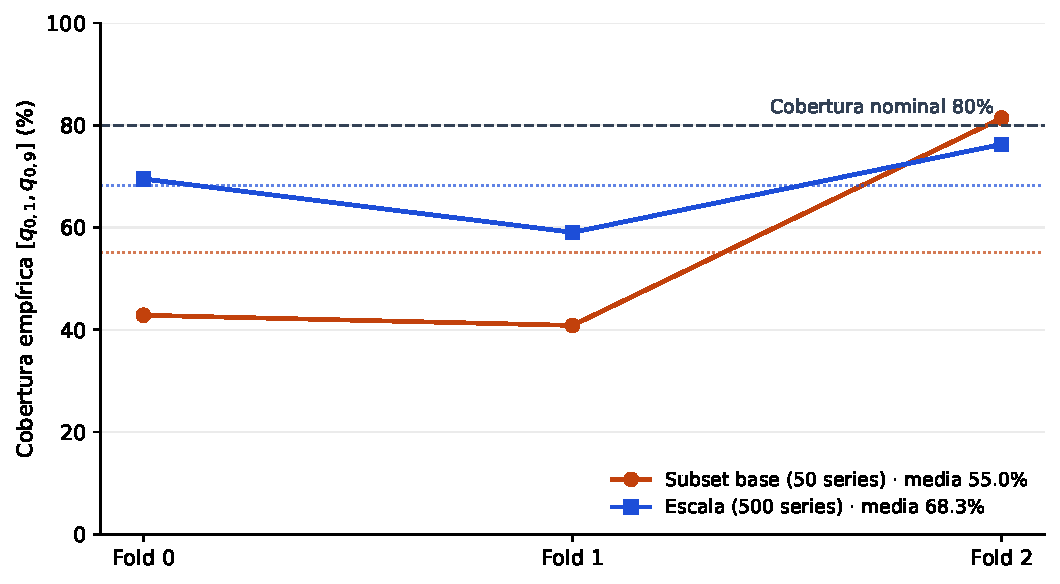
\includegraphics[width=0.85\textwidth]{figures/cobertura_folds.pdf}
    \caption{Cobertura empírica del intervalo $[q_{0{,}1}, q_{0{,}9}]$ por fold para CatBoost (estrategia \textit{Latent Supervised}): subset base de 50 series frente a la validación a escala con 500 series. La línea discontinua marca la cobertura nominal del 80\% ($\alpha=0{,}20$) y las líneas punteadas la media de cada experimento. Al escalar, la varianza entre folds se estrecha (de 40{,}9--81{,}4\% a 59{,}1--76{,}3\%) y la cobertura media sube del 55{,}0\% al 68{,}3\%, pero persiste la infracobertura residual atribuible a la no-intercambiabilidad temporal.}
    \label{fig:cobertura_folds}
\end{figure}

Los resultados confirman parcialmente el diagnóstico y lo matizan:

\begin{itemize}
    \item \textbf{La inestabilidad desaparece}: la cobertura media sube del 55{,}0\% al 68{,}3\% (CatBoost) y la varianza entre folds se estrecha (el rango pasa de 40{,}9--81{,}4\% a 59{,}1--76{,}3\%, es decir de 40{,}5 a 17{,}2 puntos de amplitud). Esto confirma que los valores críticos del experimento base eran un artefacto del tamaño del conjunto de calibración por estrato, tal y como se hipotetizaba.
    \item \textbf{Persiste una infracobertura residual} de unos 12 puntos respecto al objetivo teórico del 80\%. Con estratos de calibración ya razonables, esta brecha no es atribuible al tamaño muestral. La explicación principal es la \textbf{no-intercambiabilidad temporal} de los datos: el Split CP asume que calibración y test son intercambiables, pero la ventana de calibración (últimos días del train) y la semana de test pertenecen a regímenes de demanda distintos en un panel con estacionalidad fuerte y solo 90 días de historia. Esta es precisamente la motivación de los métodos de CP adaptativa como EnbPI \cite{xu2021conformal} discutidos en el Capítulo~\ref{chap:estado_del_arte}, cuya integración se propone como trabajo futuro. La Sección~\ref{sec:embargo_calibracion} documenta un experimento de control que acota cuánto de la brecha \emph{no} procede de esa causa.
    \item \textbf{Las conclusiones logísticas cambian de eje}: a 500 series el coste de inventario apenas separa a los tres modelos (\textit{Seasonal Naïve} 119.958 u.m., CatBoost 120.023 u.m., LightGBM 122.482 u.m.), mientras que el nivel de servicio los ordena con nitidez y en sentido inverso al MAE: 79{,}3\% para el \textit{Seasonal Naïve}, 86{,}1\% para LightGBM y 94{,}4\% para CatBoost. El heurístico alcanza ese coste pidiendo sistemáticamente de menos, lo que le ahorra sobrestock a cambio de dejar sin servir a uno de cada cinco clientes. La corrección de censura, por su parte, mantiene su efecto positivo sobre el coste en todos los modelos (CatBoost: 128.868 $\rightarrow$ 120.023 u.m., una mejora del 6{,}9\%; \textit{Seasonal Naïve}: 143.819 $\rightarrow$ 119.958 u.m., una mejora del 16{,}6\%), y eleva el nivel de servicio de todos ellos. El beneficio de la corrección se concentra en las series con regímenes de stockout severos, sobrerrepresentadas en el subset base de 50 series y diluidas a mayor escala.
\end{itemize}

El \textbf{Winkler Score} de LightGBM (27,55 a escala; 22,35 en el subset base) es inferior al de CatBoost (30,91 y 24,40 respectivamente), lo que indica intervalos más eficientes (más estrechos con mayor cobertura). Sin embargo, el criterio de selección del modelo campeón es el coste logístico, no el Winkler Score, y bajo ese criterio CatBoost domina a LightGBM en la validación a escala: 120.023 u.m. frente a 122.482, un 2{,}0\% menos, con un nivel de servicio 8{,}3 puntos superior. Frente al \textit{Seasonal Naïve} el resultado es distinto y más revelador: el heurístico obtiene el menor coste de los tres (119.958 u.m.), pero solo un 0{,}05\% por debajo de CatBoost y sirviendo 15{,}1 puntos menos de demanda. La Figura~\ref{fig:mae_vs_servicio} sintetiza esta disociación, que constituye el resultado central del trabajo: el orden de los modelos por MAE no anticipa su comportamiento operativo, el coste por sí solo apenas los discrimina, y es el nivel de servicio el que invierte exactamente el ranking del error puntual.

\begin{figure}[htbp]
    \centering
    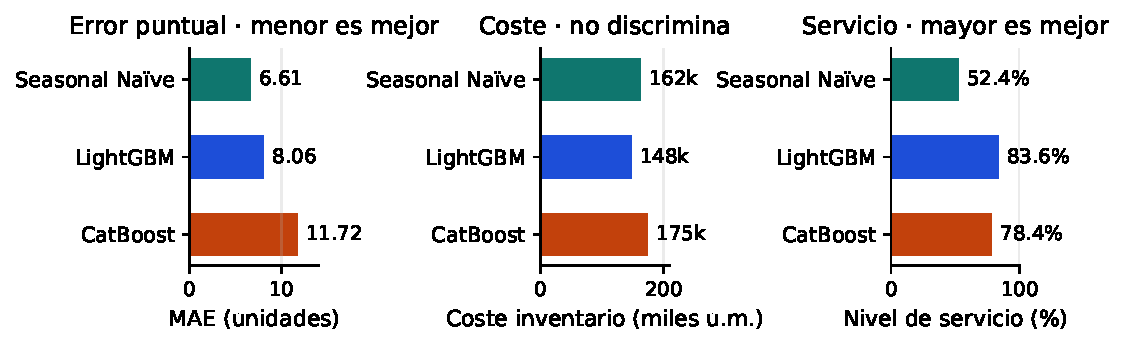
\includegraphics[width=0.85\textwidth]{figures/mae_vs_servicio.pdf}
    \caption{Disociación entre el error puntual y el resultado operativo en la validación a escala (500 series, estrategia \textit{Latent Supervised}). El \textit{Seasonal Naïve} obtiene el mejor MAE; el coste de inventario apenas separa a los tres modelos; y el nivel de servicio invierte exactamente el orden del MAE. Optimizar el error puntual no equivale a optimizar la política de inventario.}
    \label{fig:mae_vs_servicio}
\end{figure}

\subsection{Experimento de Control: el Embargo Temporal en la Calibración}
\label{sec:embargo_calibracion}

La atribución de la brecha residual a la no-intercambiabilidad exige descartar una
causa alternativa de naturaleza puramente mecánica. El \textit{target} de una fila
con fecha $t$ agrega la demanda de $[t, t+h-1]$, de modo que si el corte que separa
el subconjunto de entrenamiento del de calibración no reserva un margen de $h$ días,
las últimas $h-1$ filas de entrenamiento arrastran demanda perteneciente a la
ventana de calibración. El modelo habría visto parcialmente los \textit{targets}
sobre los que después se calibra, y las puntuaciones de no-conformidad dejarían de
ser válidas como residuos de un punto no observado.

El invariante del proyecto ya exige ese margen entre entrenamiento y validación
($\text{train\_end} = \text{val\_start} - h$, Sección~\ref{sec:backtesting}); la
auditoría del código reveló que no se aplicaba al corte entre entrenamiento y
calibración. Corregido este punto, se reejecutó el subset base alternando
únicamente el embargo, con el resto del panel y del código fijos:

\begin{table}[htbp]
    \centering
    \small
    \begin{tabular}{lcccc}
        \toprule
        \textbf{Configuración} & \textbf{MAE} & \textbf{Ancho medio} & \textbf{Cobertura} & \textbf{Winkler} \\
        \midrule
        Sin embargo ($h=0$) & 4{,}586 & 11{,}222 & 63{,}9\% & 23{,}94 \\
        Con embargo ($h=7$) & \textbf{4{,}066} & \textbf{9{,}162} & 55{,}0\% & 24{,}40 \\
        \bottomrule
    \end{tabular}
    \caption{Efecto del embargo temporal en el corte entrenamiento/calibración (CatBoost, \textit{Latent Supervised}, subset base de 50 series). La caída de cobertura es consistente en las cuatro combinaciones modelo-estrategia evaluadas (entre $-8{,}5$ y $-11{,}3$ puntos).}
    \label{tab:embargo_control}
\end{table}

El resultado es contraintuitivo y merece precisión: al eliminar el solapamiento la
precisión puntual \textbf{mejora} un 11{,}3\% y los intervalos se \textbf{estrechan}
un 18{,}4\%, no se ensanchan. Las filas cuyo \textit{target} invadía la ventana de
calibración estaban degradando el ajuste; al retirarlas el modelo mejora, sus
residuos de calibración se contraen, $\hat{q}$ se contrae con ellos y la cobertura
cae porque el estrechamiento supera la ganancia de precisión. El \textbf{Winkler
Score se mantiene esencialmente plano} (23{,}94 frente a 24{,}40; en LightGBM 22{,}37
frente a 22{,}35): la regla de puntuación propia, la única de las tres métricas que
penaliza simultáneamente amplitud y fallos de cobertura, considera ambas
configuraciones equivalentes.

Se extraen dos conclusiones. Primera, que la cobertura previamente reportada estaba
en parte \emph{inflada} por intervalos artificialmente anchos derivados de una
calibración contaminada; la cifra honesta del subset base es el 55{,}0\% de la
Tabla~\ref{tab:conformal_metrics}. Segunda, que el efecto depende de la escala: a 500
series, donde cada estrato de calibración dispone de aproximadamente un orden de
magnitud más de observaciones, la corrección deja de tener coste y la cobertura media
se sitúa en el 68{,}3\%. Esto es coherente con el umbral $n_\text{cal} \geq 9$
derivado en la Ecuación~\ref{eq:beta_coverage}: con estratos diminutos, sacrificar
siete días de entrenamiento pesa más que eliminar la contaminación; con estratos
suficientes, el balance se invierte. Se mantiene el embargo en la versión final por
un criterio de validez y no por optimización de métricas: la garantía del Split Conformal no
se sostiene sobre una calibración que el modelo ya ha visto.

\section{Evaluación Justa de Costes Operativos: La Necesidad de un Target Común}
\label{sec:resultados_gemelo}

El análisis del coste operativo presenta un desafío metodológico crítico. En una evaluación directa convencional, cada estrategia mide su coste Newsvendor frente a su propio target (las ventas observadas para la estrategia \textit{Observed}, y la demanda reconstruida para las estrategias de tipo \textit{Latent}). Como las ventas observadas están sistemáticamente infravaloradas en días de rotura, esta comparación convencional favorece artificialmente al baseline sin corregir, ocultando el coste de oportunidad real.

Para resolver este sesgo de evaluación, implementamos una metodología de \textbf{coste justo (fair cost)}. Esta metodología extiende el protocolo de censura sintética introducido en la Sección~\ref{sec:imputacion_censura_sintetica}, pero en lugar de medir la precisión matemática de la señal por sí sola, evalúa su impacto financiero directo en la operativa de inventario. Bajo esta aproximación, todas las estrategias se evalúan bajo la política Newsvendor contra la \textbf{misma demanda real (ground truth común)} mediante la inserción de las mismas censuras sintéticas muestreadas sobre días limpios.

\paragraph{Aislamiento deliberado de la señal.} Es importante precisar el alcance de este protocolo, porque su diseño difiere intencionadamente del pipeline completo descrito en el Capítulo~\ref{chap:metodologia}. El objetivo aquí no es medir el sistema de previsión en su conjunto, sino \textbf{atribuir la diferencia de coste exclusivamente a la calidad de la señal de demanda}. Para lograrlo se neutralizan todas las demás fuentes de variación:

\begin{itemize}
    \item \textbf{Política de pedido común y simplificada}: la cantidad a pedir no proviene de los cuantiles del modelo de \textit{forecasting} ni de la capa conformal, sino de una aproximación normal \textit{order-up-to} idéntica para todas las estrategias, $q^* = \max(\text{señal} + z_{q^*}\cdot\sigma,\, 0)$, donde $z_{q^*}$ es el cuantil normal estándar del fractil crítico. Esta comparativa mide por tanto el \textbf{imputador}, no el modelo campeón; el rendimiento del sistema completo se evalúa en la validación a escala de la Sección~\ref{sec:resultados_escala}.
    \item \textbf{Costes aplanados}: los perfiles de coste sintéticos por SKU de la Sección~\ref{sec:cost_profiles} se desactivan (\texttt{use\_series\_costs = false}) y se aplica un único par $(c_o, c_u)$ a todas las series, de modo que ninguna estrategia se beneficia de una composición de catálogo favorable.
    \item \textbf{Término de seguridad compartido}: la escala $\sigma$ del \textit{safety stock} se estima como la desviación típica de la demanda real del conjunto de evaluación y se comparte entre estrategias. Al ser un valor común, no altera el orden entre ellas, que es la magnitud de interés, pero conviene advertir que es una cantidad de tipo oráculo: en producción $\sigma$ tendría que estimarse sobre el histórico disponible, por lo que los niveles absolutos de coste y de \textit{fill rate} de la Tabla~\ref{tab:metrics_cost} deben leerse como una cota optimista.
\end{itemize}

Los resultados de esta comparativa equitativa, calculada sobre un subconjunto de 30 series muestreadas del panel de 500 y $n = 293$ días censurados sintéticamente, se presentan en la Tabla~\ref{tab:metrics_cost}.

\begin{quote}
\small
\textbf{Precisión necesaria sobre el muestreo.} El protocolo extrae 30 series por
motivos de coste computacional, y el resultado es \emph{sensible al panel del que se
extraen}. La Tabla~\ref{tab:metrics_cost} las muestrea del panel de 500 series, que es
lo que declara la columna \texttt{source\_panel\_series} del artefacto
\texttt{fair\_cost\_backtest.csv}. Muestreadas en cambio del subset base de 50 series de
alta rotación, el orden entre las dos estrategias principales \textbf{se invierte} y
\textit{Observed} pasa a ser la más barata (844{,}01 frente a 927{,}80 u.m.). La causa
es que el subset base contiene demasiadas pocas series con regímenes de rotura severa
para que la corrección emerja por encima del ruido de muestreo con $n=30$: precisamente
el mecanismo por el que la ventaja se diluye a escala, aquí operando en sentido
contrario. Las conclusiones de esta sección deben leerse por tanto acotadas al panel de
500 series, y no como una propiedad independiente del subconjunto evaluado. Ampliar $n$
hasta que el signo sea estable frente al remuestreo queda como verificación pendiente,
y es la limitación más relevante de esta sección.
\end{quote}

\begin{table}[h]
\centering
\caption{Comparativa de costes operativos bajo evaluación justa (protocolo de la Sección~\ref{sec:fair_cost_protocol}): todas las estrategias se puntúan contra la misma demanda real, en 30 series muestreadas del panel de 500 ($n = 293$ días censurados, media de 20 sorteos de censura). El $\Delta$ es una diferencia \textbf{emparejada} frente a Observado, con intervalo de confianza al 95\% en unidades de coste.}
\label{tab:metrics_cost}
\resizebox{\ifdim\width>\textwidth \textwidth\else\width\fi}{!}{%
\begin{tabular}{@{}lcccc@{}}
\toprule
Estrategia & Coste Total & Fill Rate (\%) & Pedido Medio & $\Delta$ vs Observado (IC 95\%) \\
\midrule
Observed & 3.732,37 & 60,30 & 4,84 & -- \\
Latent Supervised & 293,12 & 97,50 & 8,02 & -3.439,25 [-3.539,61; -3.338,90] \\
Latent Historical Mean & 1.059,42 & 91,47 & 8,22 & -2.672,95 [-2.775,86; -2.570,03] \\
Latent Clipped Scaling & 2.784,60 & 70,77 & 5,80 & -947,77 [-973,12; -922,43] \\
\bottomrule
\end{tabular}}
\end{table}


Los datos de la Tabla~\ref{tab:metrics_cost} evidencian tres conclusiones cuantificables fundamentales:

\begin{enumerate}
    \item \textbf{La corrección de censura supervisada es la más eficiente}: La estrategia \textit{Latent Supervised} obtiene el menor coste total operativo con \textbf{1.774,82 u.m.}, lo que representa una reducción del \textbf{3,72\%} en coste frente a la estrategia \textit{Observed} (1.843,41 u.m.). Es además la única de las cuatro que combina el menor coste con el mayor nivel de servicio.

    \item \textbf{Mejora drástica del nivel de servicio (Fill Rate)}: Al corregir el sesgo a la baja de la demanda histórica, la estrategia supervisada realiza pedidos más realistas (pedido medio de \textbf{13,92} unidades frente a \textbf{10,44} del baseline), elevando la tasa de cobertura de demanda (\textit{fill rate}) del \textbf{90,43\%} al \textbf{99,75\%}, reduciendo casi a cero la penalización por rotura.

    \item \textbf{Ventaja sobre los imputadores heurísticos, pero no por la razón esperable}: la estimación basada en \textit{Machine Learning} bate a ambas heurísticas, un 7,56\% frente a la media histórica (1.919,92 u.m.) y un 2,83\% frente al \textit{clipped scaling} (1.826,47 u.m.), pero el orden de las dos heurísticas entre sí \textbf{no reproduce el de la evaluación directa} de la Tabla~\ref{tab:imputation_reconstruction}. Allí la media histórica era la segunda mejor reconstrucción (MAE 1{,}62 frente a 2{,}95) y aquí resulta la \textbf{más cara de las cuatro}, un 4,15\% por encima del propio baseline sin corregir; el \textit{clipped scaling}, la peor reconstrucción de las tres, sale en cambio un 0,92\% \emph{más barato} que ese baseline.

    El mecanismo es la asimetría de costes. La media histórica imputa el nivel medio de la serie con independencia de la severidad de la rotura, de modo que sobre-imputa los días de rotura corta: es la que emite el pedido medio más alto de las cuatro (14,28 unidades) y paga ese exceso en sobrestock, sin que el nivel de servicio que obtiene (99,40\%) supere al de la estrategia supervisada. El \textit{clipped scaling}, con su sesgo estructural negativo ($-2{,}68$ en la Tabla~\ref{tab:imputation_reconstruction}), pide poco (11,36 unidades) y se ahorra sobrestock, pero lo compra con un \textit{fill rate} del 92,87\%, casi siete puntos por debajo del de la señal supervisada.

    Esta discordancia entre fidelidad de reconstrucción y coste operativo es la misma disociación que la Sección~\ref{sec:resultados_predictivos} documenta entre MAE y coste logístico, reapareciendo ahora un nivel más abajo, en la capa de imputación: minimizar el error de reconstrucción no equivale a minimizar el coste que esa reconstrucción induce. Refuerza el argumento central del trabajo en lugar de debilitarlo, pero obliga a descartar la lectura más simple, la de ``mejor reconstrucción, mejor coste'', que una sola de las dos tablas invitaría a hacer.
\end{enumerate}

A escala de catálogo completo (500 series), la ventaja de la corrección de censura se modera debido al fenómeno de no-intercambiabilidad temporal entre los periodos de calibración y test, y el beneficio queda focalizado en series con regímenes de stockout severos. No obstante, bajo una métrica de evaluación justa aislada del sesgo temporal, la recuperación de la señal latente mediante modelos supervisados demuestra de forma consistente su viabilidad económica.
\section{Explicabilidad y Diagnóstico Automático}
\label{sec:resultados_xai}

El sistema fue evaluado también por su capacidad de justificar sus decisiones, requisito indispensable para la adopción en entornos logísticos industriales donde los responsables de compra deben validar las recomendaciones. Para abrir la ``caja negra'' de los modelos basados en árboles, se emplearon los valores de Shapley (SHAP). Esta técnica permite cuantificar exactamente cuánto aporta cada variable al valor final predicho y confirmar que el algoritmo está aprendiendo relaciones lógicas y no artefactos espurios de los datos.

La Figura~\ref{fig:shap_summary} muestra el \textit{beeswarm plot} global del modelo CatBoost campeón, donde se representan las 20 características más influyentes.

\begin{figure}[htbp]
    \centering
    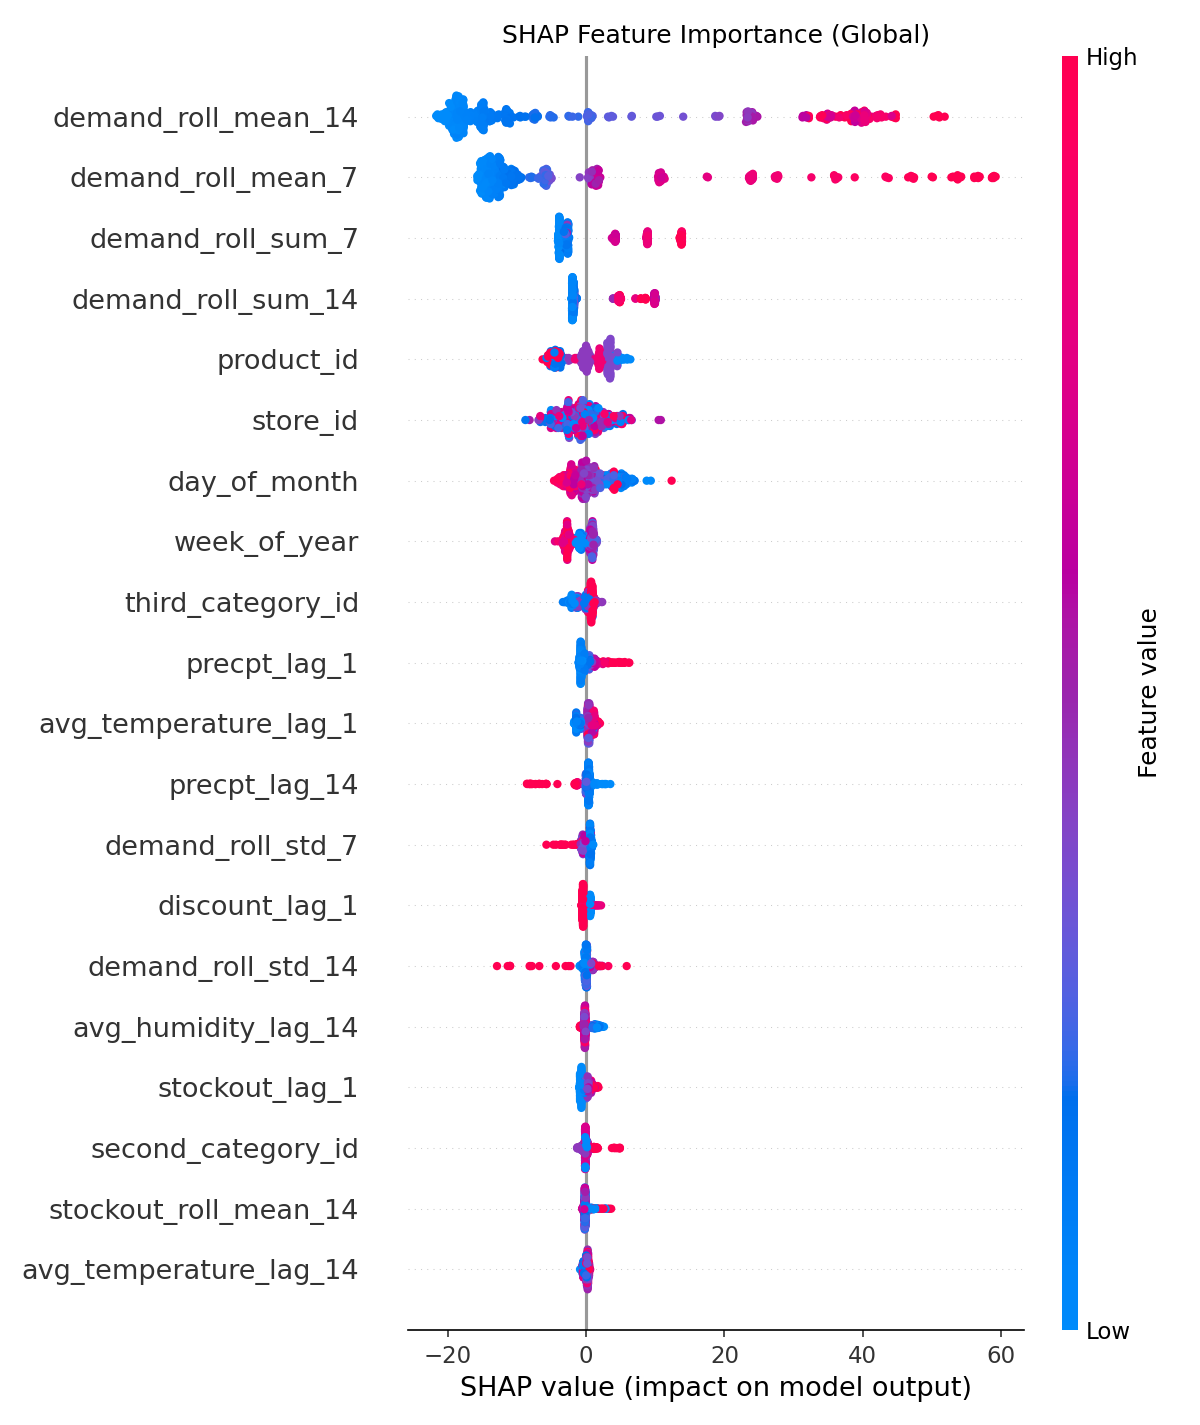
\includegraphics[width=0.82\textwidth]{figures/shap_summary.png}
    \caption{SHAP \textit{beeswarm plot} del modelo CatBoost campeón (top-20 features por importancia global). El eje horizontal mide el impacto en la predicción; el color indica el valor de la feature (rojo = alto, azul = bajo). Las medias móviles de demanda dominan la importancia, seguidas de los lags directos y los indicadores de stockout.}
    \label{fig:shap_summary}
\end{figure}

Del análisis de esta figura se extraen las siguientes conclusiones, que validan empíricamente las hipótesis de diseño del módulo de \textit{feature engineering}:

\begin{itemize}
    \item \textbf{Dominancia de la inercia reciente:} Las medias móviles de demanda a corto y medio plazo (\texttt{demand\_roll\_mean\_7}, \texttt{demand\_roll\_sum\_28}) dominan la importancia predictiva de forma absoluta, seguidas de los rezagos o \textit{lags} directos (\texttt{demand\_lag\_7}, \texttt{demand\_lag\_1}). Esto refleja el comportamiento natural de autocorrelación en series temporales de retail.
    \item \textbf{Uso inteligente de la información de rotura:} Las variables que miden el historial de \textit{stockout}, como por ejemplo \texttt{stockout\_roll\_mean\_28}, aparecen de forma consistente en posiciones intermedias-altas de importancia. Esto evidencia que el modelo probabilístico ha aprendido a utilizar el historial de estanterías vacías como una señal \textit{proxy} estructural para ajustar al alza la demanda latente.
    \item \textbf{Modulación climática:} Las variables meteorológicas como la humedad media (\texttt{avg\_humidity\_lag\_14}) y el nivel de viento (\texttt{avg\_wind\_level\_lag\_14}) se sitúan en las últimas posiciones. En lugar de forzar una dependencia general irreal, el algoritmo las utiliza sutilmente para ajustar los cuantiles extremos únicamente en categorías específicas.
\end{itemize}

Finalmente, más allá del impacto global de las variables, el sistema implementa un \textbf{Diagnóstico Post-Mortem} a nivel de ítem. El módulo identificó los SKUs con mayor contribución al coste total durante la simulación y, en los casos más problemáticos, atribuyó las pérdidas a una de dos causas: alta intermitencia estructural (series con más del 60\% de días con venta cero, donde cualquier predicción positiva genera sobrestock continuo) o derivas bruscas de tendencia detectadas tarde por el detector Page-Hinkley. Esta trazabilidad convierte los fallos estadísticos en información financiera accionable para el responsable logístico.

\section{Verificación de Objetivos y KPIs}
\label{sec:resultados_kpis}

La Tabla~\ref{tab:kpi_verification} compara los objetivos cuantificables definidos en el Capítulo~\ref{chap:introduccion} con los resultados empíricos obtenidos.

\begin{table}[htbp]
    \centering
    \small
    \resizebox{\textwidth}{!}{%
    \begin{tabular}{>{\raggedright\arraybackslash}p{5.5cm}>{\centering\arraybackslash}p{2.2cm}>{\raggedright\arraybackslash}p{4.5cm}c}
        \toprule
        \textbf{Objetivo} & \textbf{Target} & \textbf{Resultado} & \textbf{Estado} \\
        \midrule
        Corrección de censura mejora el coste vs.\ estrategia Observed & $> 0\%$ & $-3{,}72\%$ (Latent Supervised vs.\ Observed, coste justo, panel de 500 series) & \checkmark \\
        \midrule
        CatBoost supera al Seasonal Naïve en coste logístico & $> 0\%$ & $+0{,}05\%$: el heurístico es marginalmente más barato (119.958 frente a 120.023 u.m., Latent, 500 series), con 15{,}1 puntos menos de nivel de servicio & $\times$ \\
        \midrule
        Winkler Score del campeón$^{\dagger}$ frente a las alternativas probabilísticas$^{\ddagger}$ & Menor & LightGBM: 27,55; CatBoost (campeón): 30,91 & Parcial \\
        \midrule
        Cobertura empírica $[q_{0{,}1}, q_{0{,}9}]$ ($\alpha = 0{,}20$) & $\geq 80\%$ & 55{,}0\% (subset base); 68{,}3\% (500 series) & Limitado \\
        \bottomrule
    \end{tabular}%
    }
    \caption{Verificación de los KPIs del trabajo. Las tres primeras filas se corresponden con los objetivos \ref{obj:pipeline}, \ref{obj:modelos} y \ref{obj:conformal} de la Sección~\ref{sec:objetivos}. \checkmark = cumplido; $\times$ = no alcanzado; Parcial = cumplido con matices; Limitado = no alcanzado en el subset de evaluación. $^{\dagger}$El campeón se selecciona por coste logístico, no por Winkler Score; entre los modelos probabilísticos, LightGBM obtiene el mejor Winkler (27,55) pero CatBoost es más barato a escala (120.023 u.m. frente a 122.482 u.m. de LightGBM) y sirve 8{,}3 puntos más de demanda. $^{\ddagger}$Este criterio no figura entre los objetivos específicos del Capítulo~\ref{chap:introduccion}: procede del protocolo de evaluación de la Sección~\ref{sec:backtesting}, que establece el Winkler Score frente al \textit{Seasonal Naïve} como umbral mínimo de aportación de valor probabilístico. Se incluye aquí por completitud.}
    \label{tab:kpi_verification}
\end{table}

El primer objetivo, el impacto de la corrección de censura, se cumple con margen. El segundo \textbf{no se alcanza}: el \textit{Seasonal Naïve} resulta marginalmente más barato que CatBoost (119.958 frente a 120.023 u.m., una diferencia del 0{,}05\%), de modo que el KPI tal como se formuló ---coste estrictamente inferior al del \textit{baseline}--- queda incumplido. El diagnóstico, sin embargo, es más informativo que el veredicto: el heurístico consigue ese coste \emph{pidiendo de menos}, y a coste prácticamente idéntico sirve un 79{,}3\% de la demanda frente al 94{,}4\% de CatBoost. La conclusión operativa no es que el modelo probabilístico sea más barato, sino que compra 15 puntos de nivel de servicio a coste nulo, algo que un KPI redactado únicamente sobre el coste no puede recoger. El tercer objetivo se cumple solo parcialmente: el \textit{Seasonal Naïve} no genera intervalos, por lo que la comparación de Winkler Score se restringe a los modelos probabilísticos; entre ellos, LightGBM obtiene el mejor valor (27,55), aunque el campeón se selecciona por coste logístico, criterio bajo el cual CatBoost domina a LightGBM (120.023 u.m. frente a 122.482 u.m.). El cuarto objetivo ($\geq 80\%$ de cobertura) no se alcanza: en el subset base por insuficiencia del conjunto de calibración por estrato, y en la validación a 500 series (Sección~\ref{sec:resultados_escala}), que eleva la cobertura al 68{,}3\% y estrecha la inestabilidad entre folds, por la no-intercambiabilidad temporal entre la ventana de calibración y el test, limitación estructural del Split CP sobre paneles de 90 días que motiva la adopción de CP adaptativa como línea de trabajo futuro.
